
\subsection{The transient current technique}

In transient current experiments, also referred to as time-of-flight experiments,
 time-resolved currents are recorded that are induced on a read-out electrode by the drift of free charge carriers in an externally applied electric field. 
The sensor current induced by moving charges is elegantly formulated by the Shockley-Ramo theorem\,\cite{1686997}.
It makes use of a \textit{weighting potential} $\Phi_{\textrm{w}}$ which describes the coupling of a charge to an electrode.
The weighting potential therefore depends on the electrode configuration. 
Note that the weighting field $E_\textrm{w}$ is not to be confused with the electric field $E$: $\vect{\nabla}\Phi_{\textrm{w}} = - \vect{E}_{\textrm{w}} \neq - \vect{E}$.
With the number of drifting charges $Q$ and their trajectory $\vect{r}(t)$, the induced current reads

\begin{equation}
 i(t) = Q(t) \vect{\nabla}\Phi_{\textrm{w}} \frac{\dd}{\dd t}\vect{r}(t) = - Q(t) \vect{E_{\textrm{w}}} \vect{v}. 
\end{equation}

\noindent
In a parallel plate configuration the weighting field reduces to be $\vect{E_{\textrm{w}}} =  -\frac{\dd \Phi_{\textrm{w}}}{\dd x}= -1/d$ with the plate distance $d$. 
For a one-dimensional charge drift in an electric field of constant strength and with $Q(t) = \e \cdot N(t)$, the current density reads

\begin{equation}
  i(t) = \e \cdot N(t) \cdot \vdrift / d.
 \label{eq:ramo}
\end{equation}

The TCT provides direct way to derive the transit time of a localised charge cloud, i.e.~the time a charge cloud requires to drift through a crystal,
 from the time difference between the rising and the falling edge. 
This technique is usually, and also in this work, performed in a electrode-semiconductor-electrode structure.
Localised creation of free charges close to the electrode surface is realised by using highly ionising $\alpha$-particles with short penetration depth
 from an ${}^{241}\textrm{Am}$ source. 
Bragg-simulations based on NIST data \cite{NIST} show a penetration depth of approximately $\SI{10}{\micro\meter}$ for an $\alpha$-particle energy of $\SI{4.7}{\MeV}$,
 which is small compared to the sample thicknesses of about $\SI{500}{\micro\meter}$ used in this work. 
Transit times are of the order of few nanoseconds for such crystal sizes.
The drift of free charge carriers depends on the material's crystal properties and on the release mechanism from the initial charge cloud. 
Therefore, if the current is read with wide bandwidth, charge carrier properties and details about the release mechanism are accessible from the current pulse characteristics. 


\subsection{The measurement set-up}
The samples under test (SUT), which are referred to as \textit{S52}, \textit{S57}, and \textit{S79} for later reference, have been produced by chemical vapour deposition process
 by Element Six Ltd (E6) \cite{E6}.
The scCVD diamond samples have an area of $4.7 \times \SI{4.7}{\milli\meter^2}$
 and thicknesses of $d_{\textrm{S52}} = \SI{515}{\micro\meter}$, $d_{\textrm{S57}} = \SI{530}{\micro\meter}$, and $d_{\textrm{S79}} = \SI{529}{\micro\meter}$.
The dislocation and impurity densities are of the order of $\le \SI{2e14}{\centi\meter^{-3}}$. 
DDL quotes a nitrogen incorporation of $<\SI{1}{\ppb}$.
The leakage current is less than $\SI{7}{\pico\ampere}$ for $E = \pm \SI{1.1}{\volt/\micro\meter}$. 
In present scCVD diamond specimen, trapping times larger than $\SI{30}{\nano\second}$ have been realised \cite{pernegger:073704}. 

\begin{figure}[tb]
  \centering
  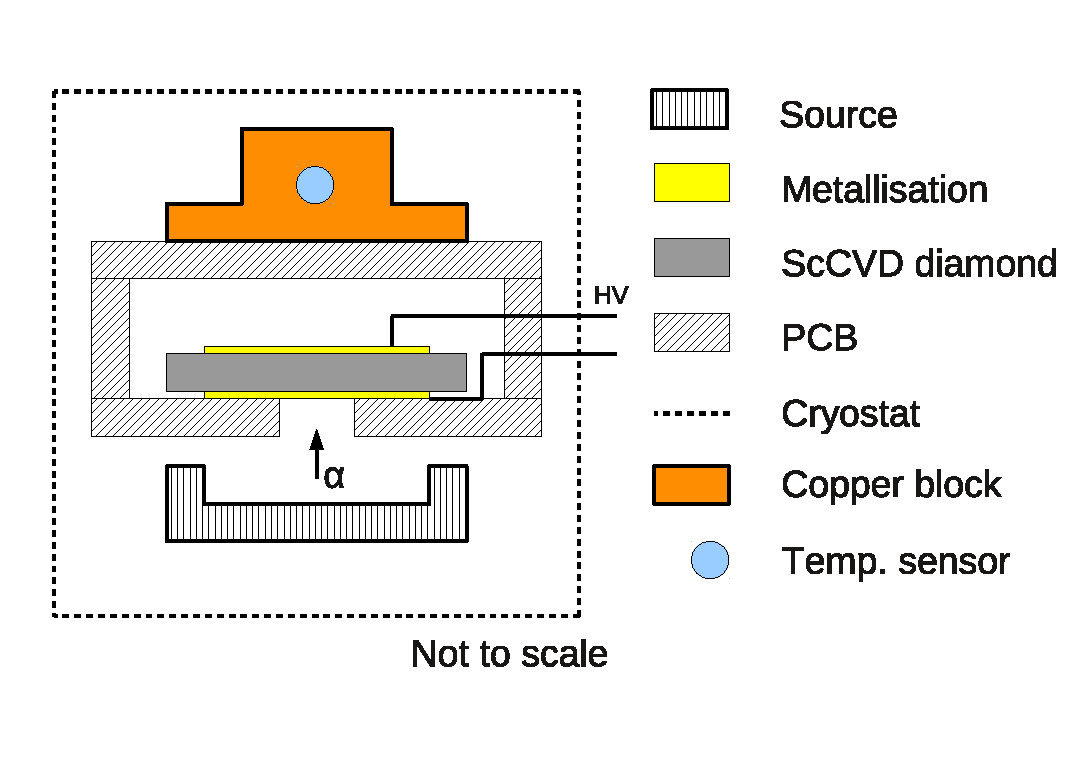
\includegraphics[trim=0cm 1.5cm 0cm 0.5cm, clip=true,width=0.45\textwidth]{./figures/diamond_collimator4.eps}

  \caption{The measuring unit is detailed. The thermal heater is omitted and is located behind the copper block.}
  \label{fig:SETUPtct}
\end{figure} %FIXME cryostat should read innver vacuum chamber in the plot

The set-up used for the presented measurements consists of a measuring unit, a digital oscilloscope, a thermal heater, and a liquid helium cryostat comprising an inner vacuum chamber (IVC). 
The measuring unit consists of a PCB sensor holder providing a backside contact to ground and a $\SI{50}{\ohm}$ read-out line, which also serves as high-voltage contact. 
The cryostat holds the liquid helium, the measuring unit is situated in the IVC,
 which has been evacuated prior to the measurements and then filled with helium gas to a pressure of $\sim\SI{5e-2}{\milli\bar}$.
This provides an excellent thermal contact whilst keeping the breakdown voltage high enough. 
Furthermore, a calibrated CERNOX temperature sensor at close vicinity to the SUT is thermally coupled to the PCB via a copper block. 
The sensor holder has a hole of $\textrm{\O} = \SI{1}{\milli\meter}$ at the bottom, collimating the $\alpha$-particles from the ${}^{241}\textrm{Am}$ source
 and ensuring that they impinge the sensor only within the metallised area.
A sketch of the cross section of the measuring unit is shown in Fig.~\ref{fig:SETUPtct}. %1 in reference \cite{ jansen:173706}.
The $\alpha$-particles emitted from the ${}^{241}\textrm{Am}$ %source have an energy of $\SI{5.48}{\MeV}$. 
reach the bulk with $\sim \SI{4.7}{\MeV}$,
 corresponding to $\num{3.5e5}$ created electron-hole (e-h) pairs in the diamond sample under the assumption of an average e-h pair creation energy of $\SI{13.25}{\eV}$\cite{4329650}. 
At the lowest absolute applied bias voltage ($\SI{30}{\volt}$), the sensor capacity is charged with $\SI{6e-11}{\coulomb}$ on the electrodes,
 or $\SI{3.7e8}{\e}$, which is much larger than the number of induced e-h pairs per $\alpha$-particle. 
Hence, the produced free charge carriers do not change significantly the electric field in the bulk region. 

Figure~\ref{fig:SETUPtct2} shows the electrical schematics of the set-up. 
The high voltage is applied to the top contact and is AC-coupled to the amplifier via a $\SI{1}{\nano\farad}$ capacitor. 
The electrical connection to the amplifier, which is located outside of the cryostat, is realised via a vacuum-tight feedthrough. 
As electron-hole (e-h) pairs are created close to the bottom contact,
 one charge carrier type is collected there almost instantly,
 whilst the other drifts through the entire bulk to reach the top contact. 
Hole (electron) induced currents are read if a negative (positive) bias voltage is applied to the top contact.

\begin{figure}[t]
  %\centering
  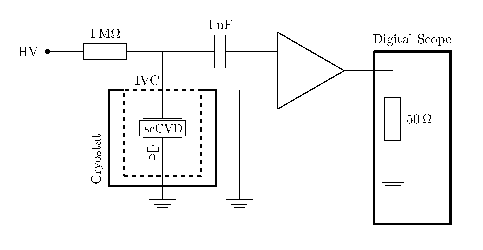
\includegraphics[width=0.45\linewidth]{./figures/circuit2}

   \caption{The electrical schematics of the TCT set-up are shown. 
   The diamond sample is situated in a vacuum chamber with electrical connections to the outside. 
   The vacuum chamber resides within the liquid helium cooled  cryostat.}
   \label{fig:SETUPtct2}
\end{figure}

A $\SI{2}{\giga\hertz}$ bandwidth, two-staged, bipolar transistor amplifier %with an amplification factor of $A_{\textrm{amp}} = (138\pm 7) $ at $\SI{3.3}{\pico\farad}$ input capacitance,
 is used to amplify the signal before it is read via an oscilloscope. 
The minimum resolvable rise time with a $\SI{2}{\giga\hertz}$ amplifier is $\SI{180}{\pico\second}$. 
The cut-off frequency at $\SI{-3}{\decibel}$ within a RC-circuit is $f_{\textrm{cut}} = 1/(2\pi R_{\textrm{in}} \left( C_{\textrm{d}}+C_{\textrm{stray}}\right))$. 
Including stray capacitances $f_{\textrm{cut}}\approx \SI{1}{\giga\hertz}$ is estimated. 
The signal from the read-out electrode is read via a $\SI{1.6}{\meter}$ long UT-85 cable to bring the signal out of the cryostat and via a 3.15\,m high quality coax-cable outside of the cryostat
 towards the oscilloscope.
The digitalisation is realised via a LeCroy\,WavePro\,7300A with $\SI{3}{\giga\hertz}$ analogue bandwidth at a sampling rate of $\SI{10}{\giga\sample/\second}$. 
Note that neither a bandwidth limitation nor filtering has been used. 
Only at small signal-to-noise ratios ($\textrm{SNR}<9$), i.e.~at low bias voltages where the rise times are $> \SI{2}{\nano\second}$, the bandwidth was limited to $\SI{200}{\mega\hertz}$,
 affecting the length of the current pulse by less than 1\,\%. 
In summary, the read-out system provides a sufficiently wide analogue bandwidth in order to resolve features in the current pulse of down to 360\,ps. 






\subsection{Data acquisition}

The oscilloscope's trigger settings were chosen such that individual pulses are recorded, when the pulse amplitude exceeds a certain threshold of few millivolt in coincidence with a
 signal width $> \nicefrac{2}{3}$ of the actual width.
The combination of the two conditions reduced the trigger rate of shot noise induced triggers to effectively zero without cutting any signal
 whilst maintaining a short measurement duration of a few minutes per voltage-temperature pair. 

For every given pair of temperature and bias voltage setting, 300 pulses were recorded within a time window of $\SI{200}{\nano\second}$ . 
In the offline analysis the individual signals are corrected for trigger jitter and combined to form an average pulse. 
Only signals with an $\textrm{SNR}> 3$ are considered in order to
 reject pick-up triggers induced e.g.~by other equipment in the laboratory. 

